\chapter{系统需求与架构分析}
\section{需求分析}
前两章已分别阐述三类核心难题与CHESCA三路动作生成技术：基线稳健但自适应不足、纯学习方法性能潜力大但难以安全落地、实验管理分散且决策过程不透明。本章的任务是将上述问题转化为系统需要完成的功能与技术要求。参考同类毕业论文先需求后架构的组织方式\cite{vue2024,xupengtao2020,springboot2024,wangyonghe2016}，本章从三类用户视角切入，依次展开功能需求、非功能需求与架构设计。

首先分析用户角色。能源管理者关注成本节约与削峰效果，偶尔查看决策轨迹；算法研究者需要配置参数、批量执行实验、比较KPI并追踪残差细节；系统管理员负责账号、数据版本与存储运维。已有平台多停留在数据采集展示与阈值报警阶段，缺乏任务调度、版本追踪与决策解释能力，这正是本系统需要弥补的功能缺口。

\subsection{系统功能性需求分析}
系统功能划分为四个部分：系统管理、数据管理、算法与实验管理、可视化分析。

（1）系统管理。包括用户与权限管理、通知与反馈功能。后台支持用户的录入、编辑与查询，并按权限组分配菜单；管理员发布通知后用户端即时推送；问题反馈直达后台，形成``使用—改进''闭环。密码加密存储，上传文件执行白名单校验，接口层过滤SQL注入与XSS攻击。

（2）数据管理。以CityLearn数据集为核心\cite{citylearn2020,citylearn2024,gymnasium2024}，管理社区、建筑、设备与时序数据。支持数据集导入与CSV导出，记录数据集版本、时间范围与建筑数量；数据集目录维护候选数据集及其兼容性标识，任务提交前自动校验动作空间匹配性，不兼容时直接拦截，避免不合规数据进入评估流程。

（3）算法与实验管理。算法库登记可执行脚本（基线控制与残差强化学习两类入口）；任务记录状态与展示名称；配置以键值形式存储残差系数、掩码、安全开关、训练与评估数据集及模型快照。界面支持新增任务、修改参数与删除任务，便于直观比较不同参数配置。日志按任务隔离，标准输出与结构化结果文件一并归档，解析失败时保留原始行并标注原因。

（4）可视化分析。提供三类视图：KPI对比（柱状图与雷达图，呈现成本、碳排放、峰值、爬坡与舒适度的权衡关系）、时序曲线（负荷、电价、SOC、室温）与决策轨迹（基线、残差、掩码、投影的逐步展示）。设计重点不在于视觉效果，而在于使``控制决策的依据''有据可查。

系统功能结构如图\figref{功能模块图}所示。
\begin{figure}[htb]
    \centering
    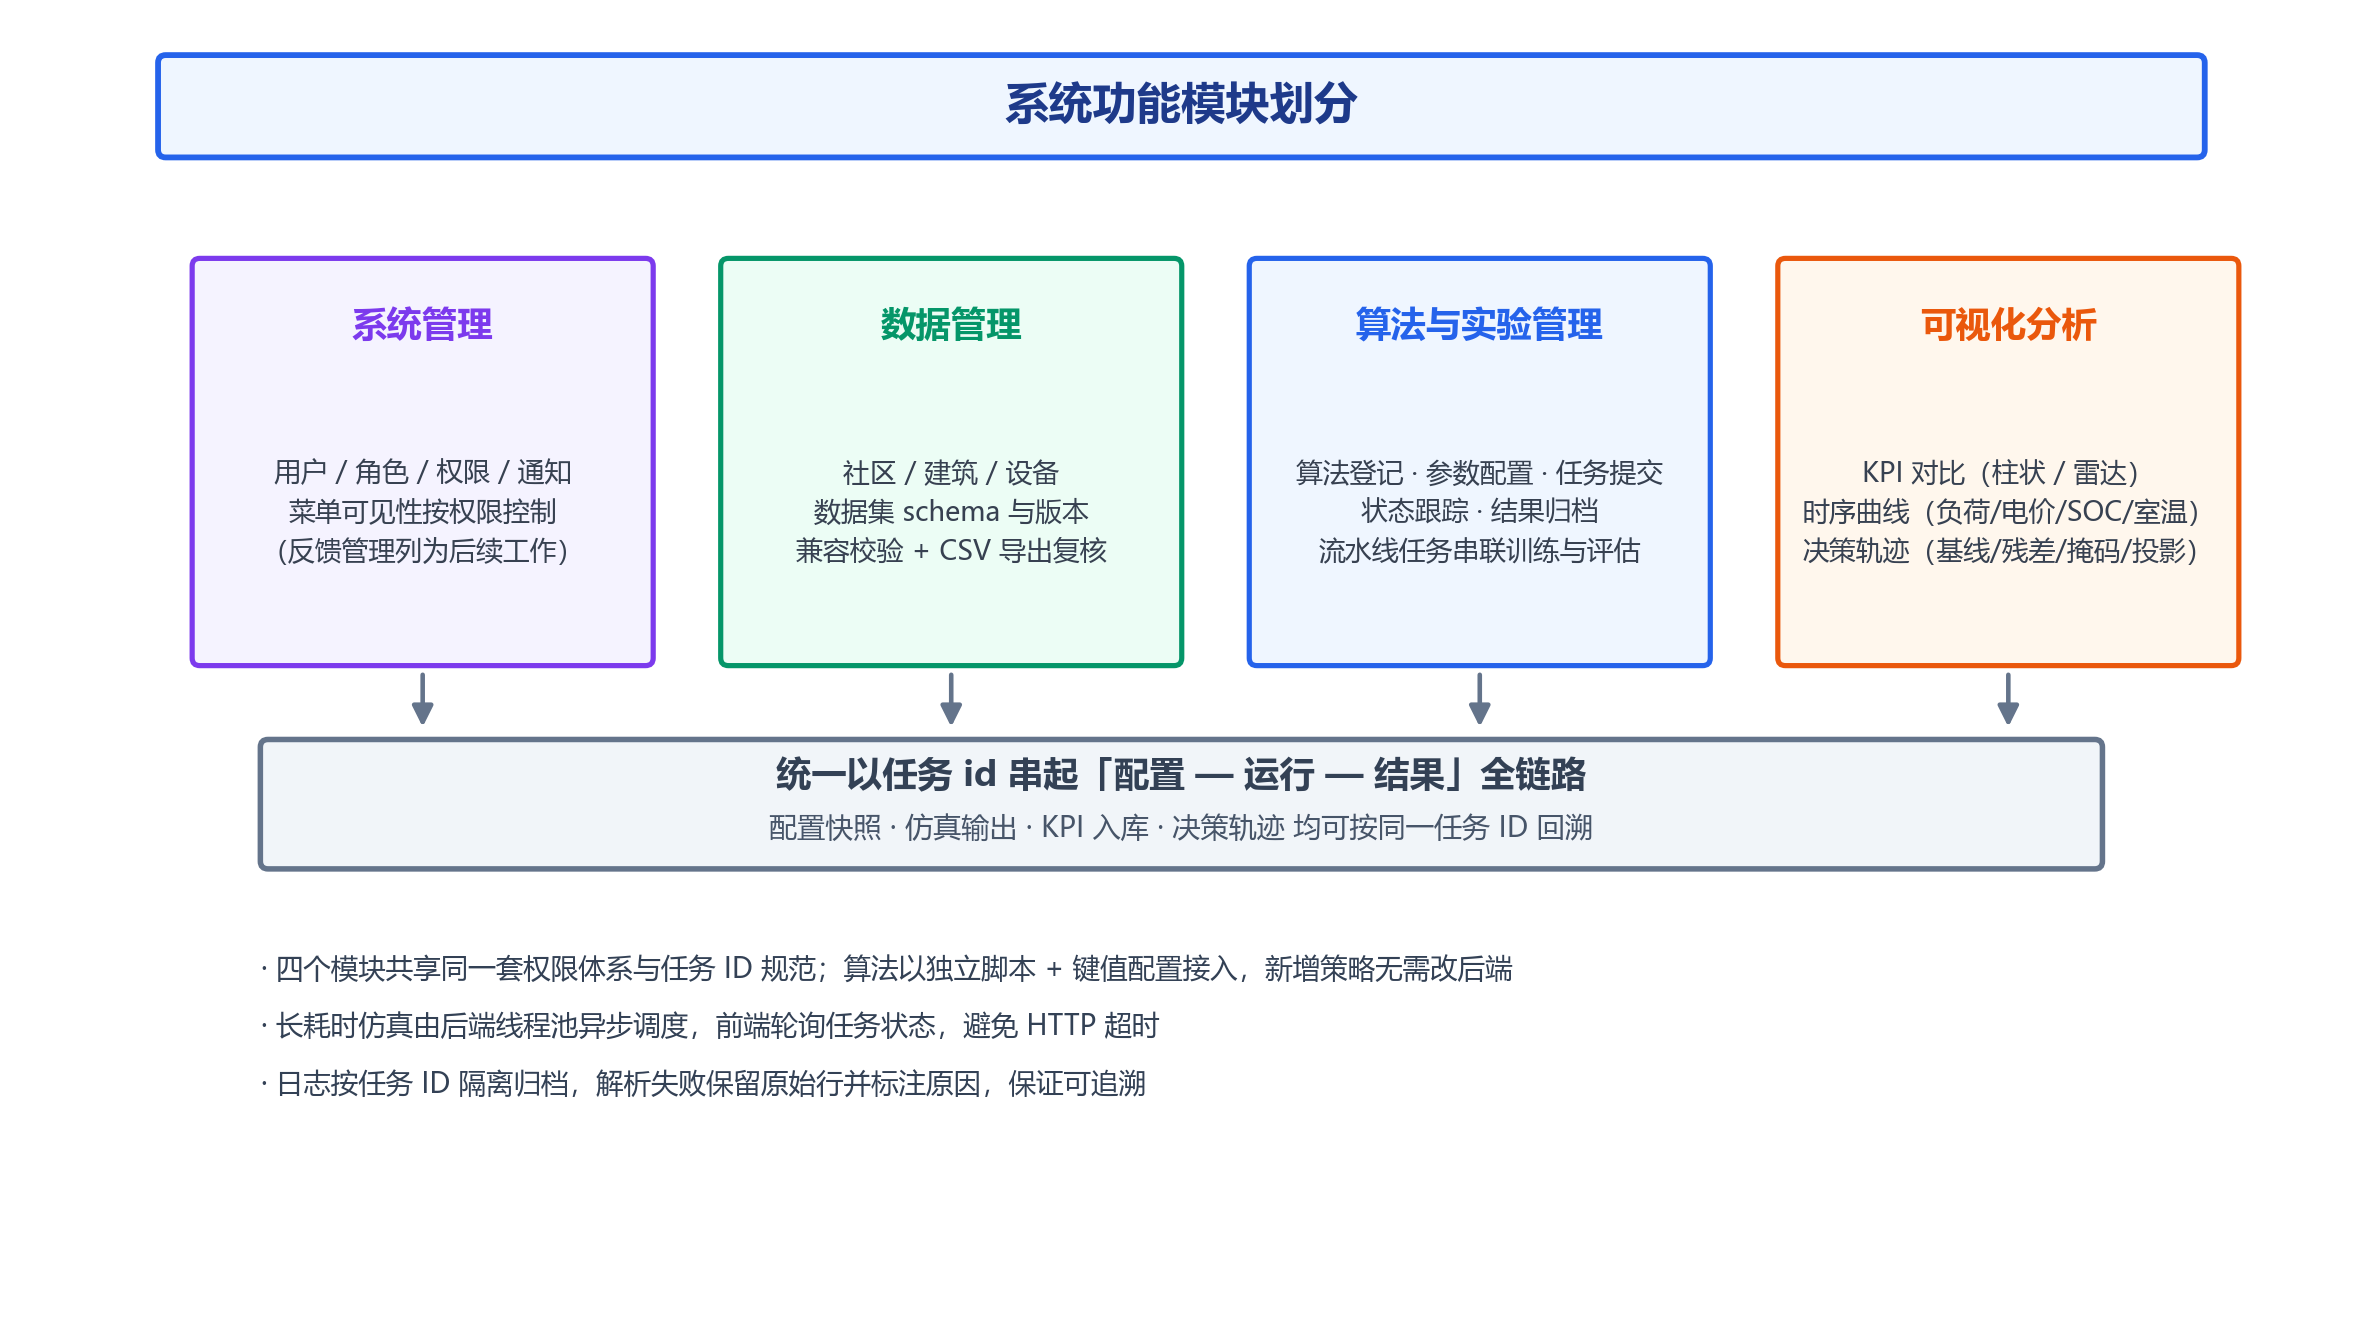
\includegraphics[width=0.92\textwidth]{./images/pictures/功能模块图.png}
    \centering\bicaption{功能模块图}{Functional modules}
    \label{功能模块图}
\end{figure}

\subsection{系统非功能性需求分析}
（1）安全性：权限控制防止越权访问，密码加密存储，上传执行白名单校验，接口过滤注入与脚本攻击，MySQL提供高可靠存储\cite{mysql2024}。

（2）兼容性：系统采用浏览器端渲染，ECharts在Chrome、Edge、Firefox中的表现略有差异\cite{echarts2024}，设计时按最低版本对齐，布局采用Element UI栅格系统\cite{elementui2024}，避免使用私有CSS特性。

（3）可扩展性：算法以独立脚本加键值配置方式接入，新增策略无需修改后端代码；接口遵循RESTful规范\cite{springboot2024}；数据格式标准化并附完整注释，便于后续扩展储能、光伏、电动汽车等设备类型。日志字段先行固化（见4.2节），后续接入ELK/Loki\cite{elk2024}时无需返工。

\section{系统架构设计}
系统采用B/S四层架构：浏览器层、前端Web服务层、后端应用层与数据存储层，如图\figref{系统架构图}所示。
\begin{figure}[htb]
    \centering
    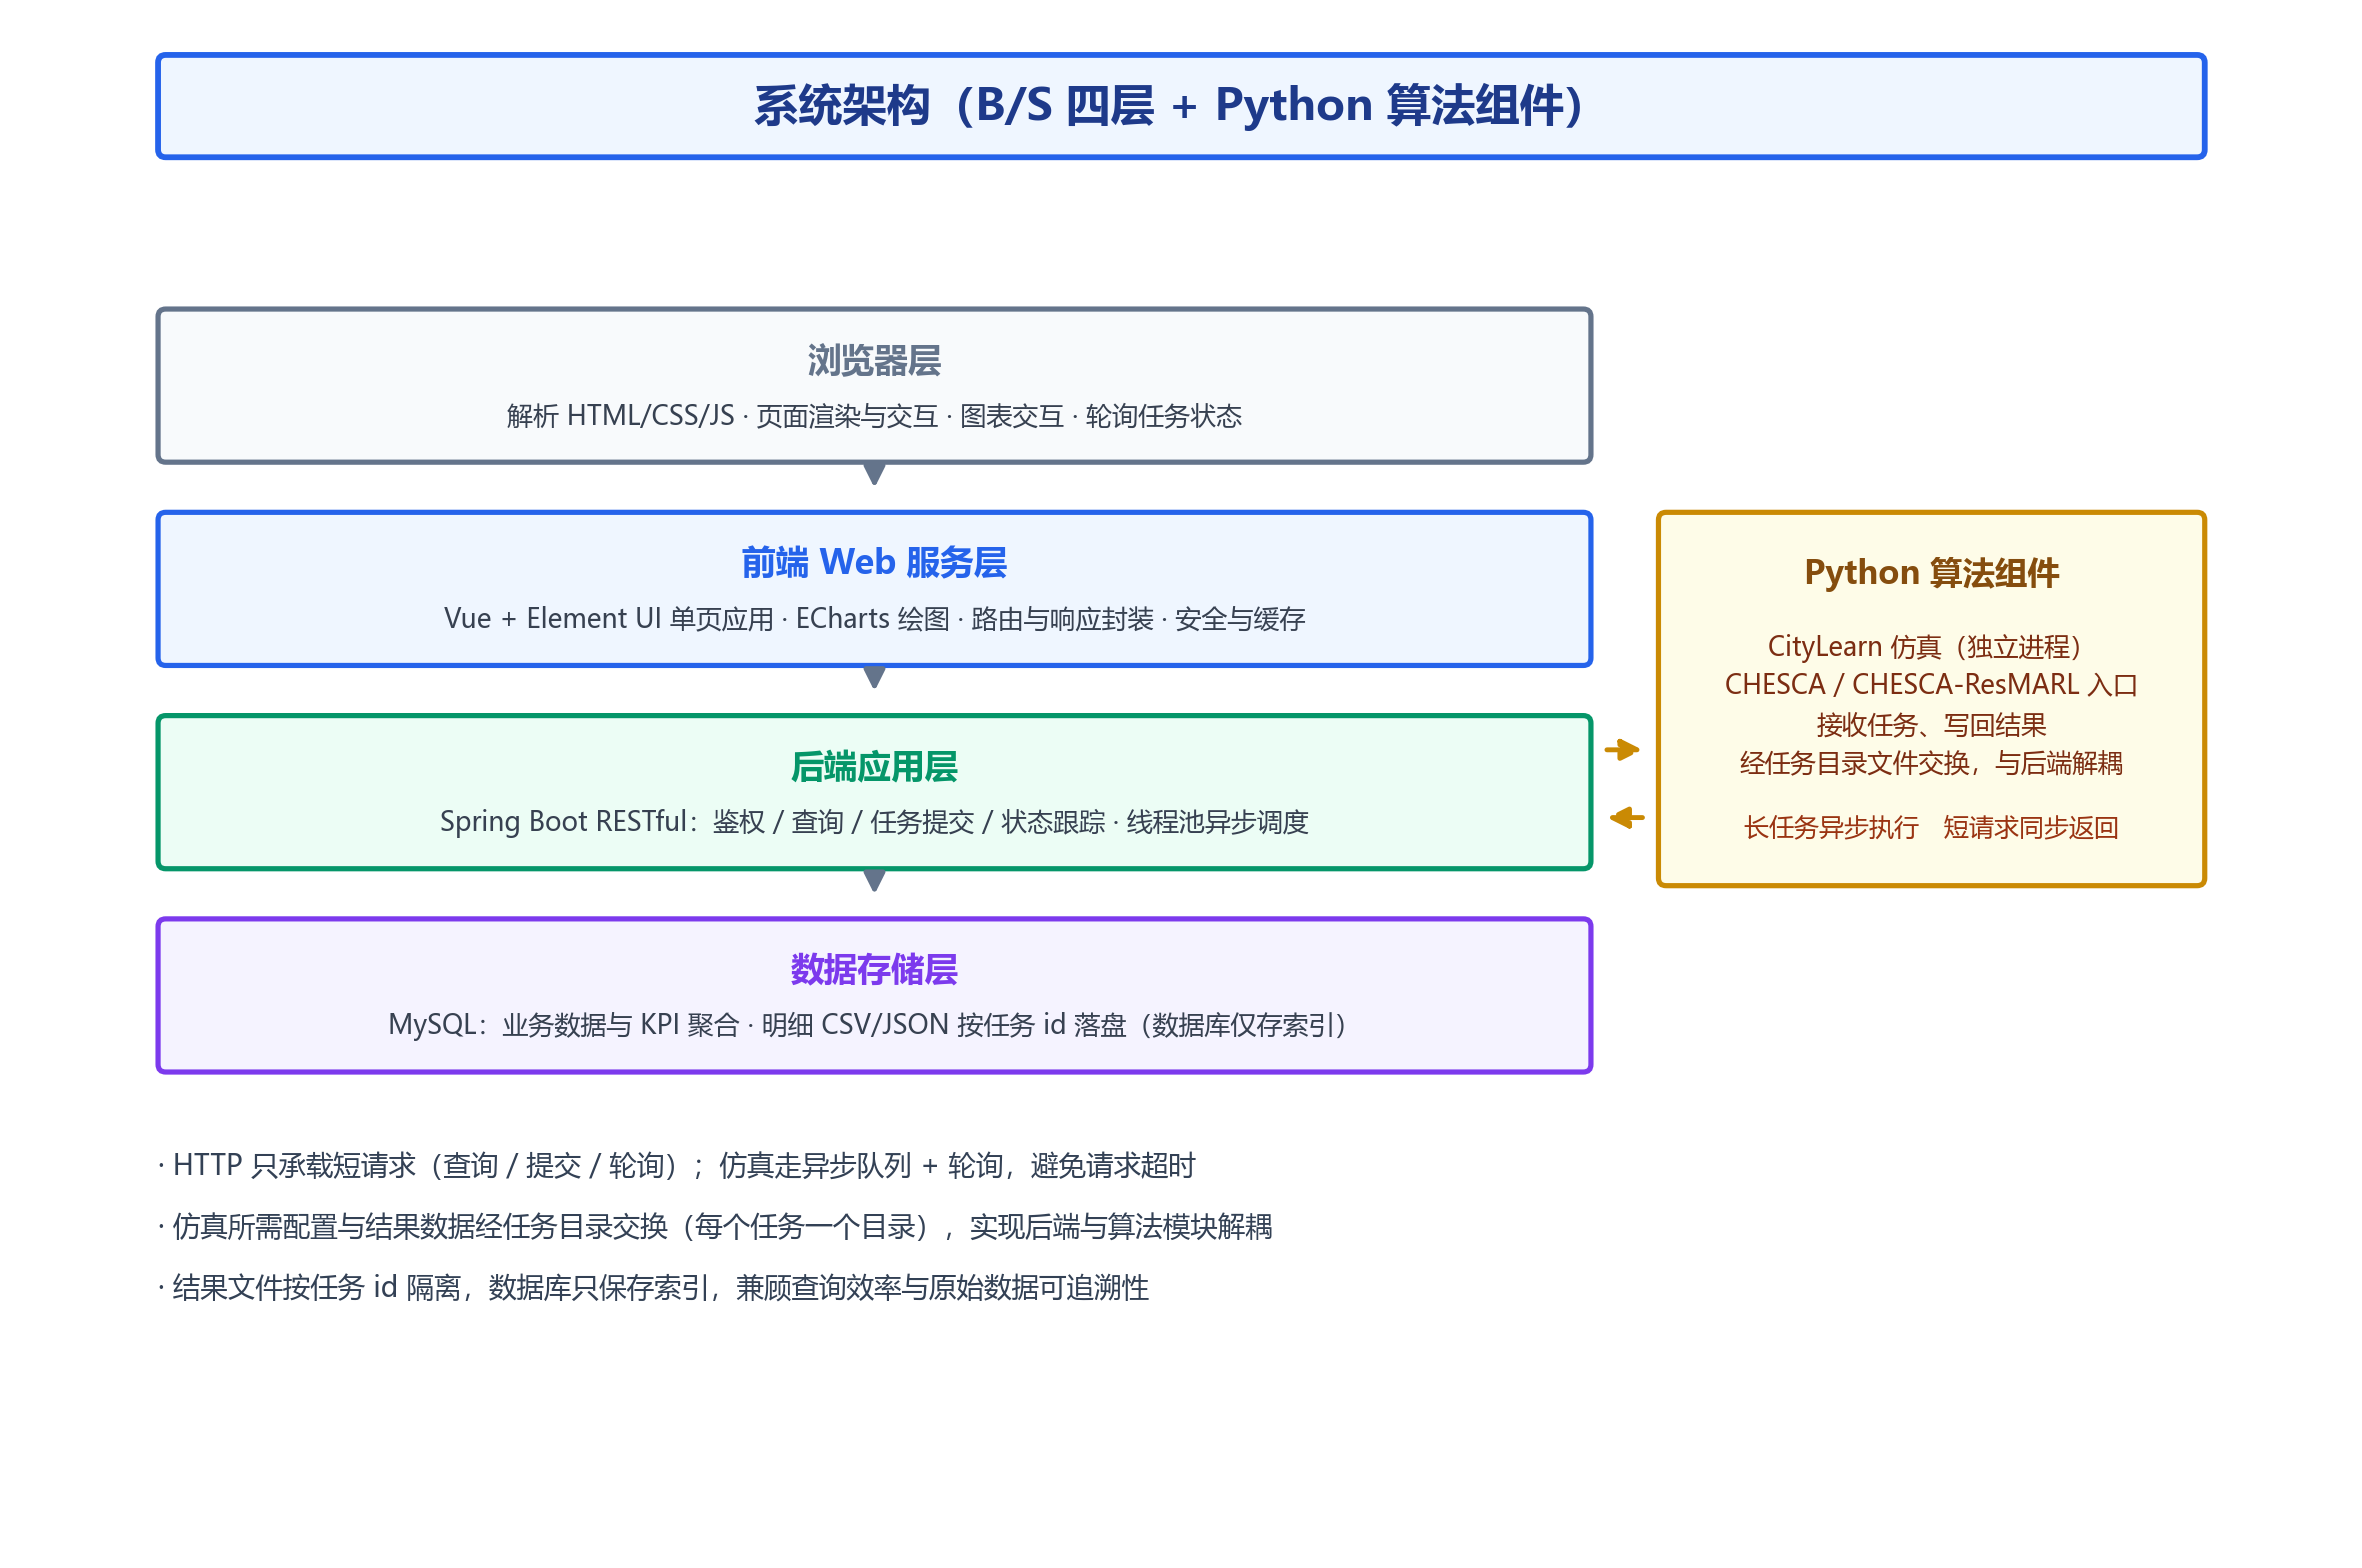
\includegraphics[width=0.85\textwidth]{./images/pictures/系统架构图.png}
    \centering\bicaption{系统架构图}{System Architecture Diagram}
    \label{系统架构图}
\end{figure}

（1）客户端浏览器：负责解析HTML/CSS/JS，渲染页面并执行交互逻辑，管理缓存与隐私数据。

（2）前端Web服务：基于Vue与Element UI构建单页应用\cite{vue2024,xupengtao2020,elementui2024}，采用ECharts绘制KPI与轨迹图表\cite{echarts2024,wangzhiwen2020}。Vue的响应式绑定与组件化机制适用于复杂动态界面开发\cite{xupengtao2020}，Vue、Element UI与ECharts的组合在项目管理平台中已有成熟应用先例\cite{wangzhiwen2020}。该层接收HTTP请求、按路由转发并封装响应，同时承担安全与缓存职能。长耗时任务不阻塞HTTP连接，由前端轮询任务状态。

（3）后端应用服务：基于Spring Boot提供RESTful接口\cite{springboot2024}，负责鉴权、查询、任务提交与状态跟踪，其自动配置与起步依赖机制大幅简化了企业级应用开发\cite{wangyonghe2016}。长耗时仿真任务异步进入队列，遵循``长任务异步、短请求同步''原则，避免请求超时。

（4）数据存储：数据库存储业务数据与指标聚合结果\cite{mysql2024}，基于Java与MySQL的数据库管理系统设计是此类业务系统的常规做法\cite{ouyangguixiu2022}；Python算法组件以独立进程运行CityLearn仿真\cite{citylearn2020,gymnasium2024}，通过HTTP/REST接口接收Java端下发的仿真任务，仿真所需的配置与结果数据经任务目录中的文件交换，实现后端与算法模块的解耦。明细时序数据与结果文件按任务目录落盘，数据库仅保存索引，兼顾查询效率与原始数据可追溯性。

\section{功能模块设计}
\subsection{系统管理模块}
涵盖用户、角色、权限与通知管理。用户管理页面提供用户的录入、编辑、查询与启停维护；角色与权限组控制菜单可见性（如任务列表入口仅对有权限用户可见）；通知以任务完成未读提醒的形式落地，与任务状态联动；问题反馈直达后台，形成``使用—改进''闭环。

\subsection{数据管理模块}
管理社区、建筑、设备与数据集版本。以数据集为单位记录建筑数量、时间步数与兼容性标识，为仿真任务提供统一输入；CSV导出功能支持离线复核。

\subsection{算法与实验管理模块}
覆盖算法登记、参数配置、任务提交、状态跟踪与结果归档。算法参数配置页面以结构化分组表单维护各算法的可配置参数，并支持以在线代码编辑器直接查看与编辑脚本；残差系数、掩码、安全开关与模型文件在提交时进行校验并生成配置快照；任务由后端线程池异步调度执行；任务列表页面支持任务的分页查询、进度轮询、标准输出与错误日志查看；流水线任务支持将多个步骤（如训练与评估）串联为子任务序列。

\subsection{可视化分析模块}
指标对比读取指标汇总数据，支持多任务横向比较与雷达图展示；时序视图按建筑与时间维度绘制负荷、电价、SOC与室温曲线；轨迹视图逐步呈现基线、残差、掩码与投影结果。全系统统一采用任务标识，保证配置、仿真与结果全链路可追溯。核心业务流程为：用户登录后选择数据集与算法，配置参数并提交任务；调度器写入配置并调用Python执行；任务完成后解析指标入库，前端跳转至分析页面。

\section{数据库概念设计}
数据库采用MySQL 8.0 InnoDB引擎，字符集为\texttt{utf8mb4}。数据按业务功能分为三类：第一类为建筑与环境时序数据，承载各建筑的分时观测以及天气、电价、碳强度等外部环境信息；第二类为运行结果数据，承载算法脚本登记、仿真任务状态与各项评价指标；第三类为配置与目录数据，承载算法可调参数与数据集登记信息。

表间联系为：脚本与任务为1:N关系；任务与指标及结果文件为1:N关系；数据集与任务为1:N关系；各类时序数据按时间步号逻辑对齐。如图\figref{数据库E-R图}所示。
\begin{figure}[htb]
    \centering
    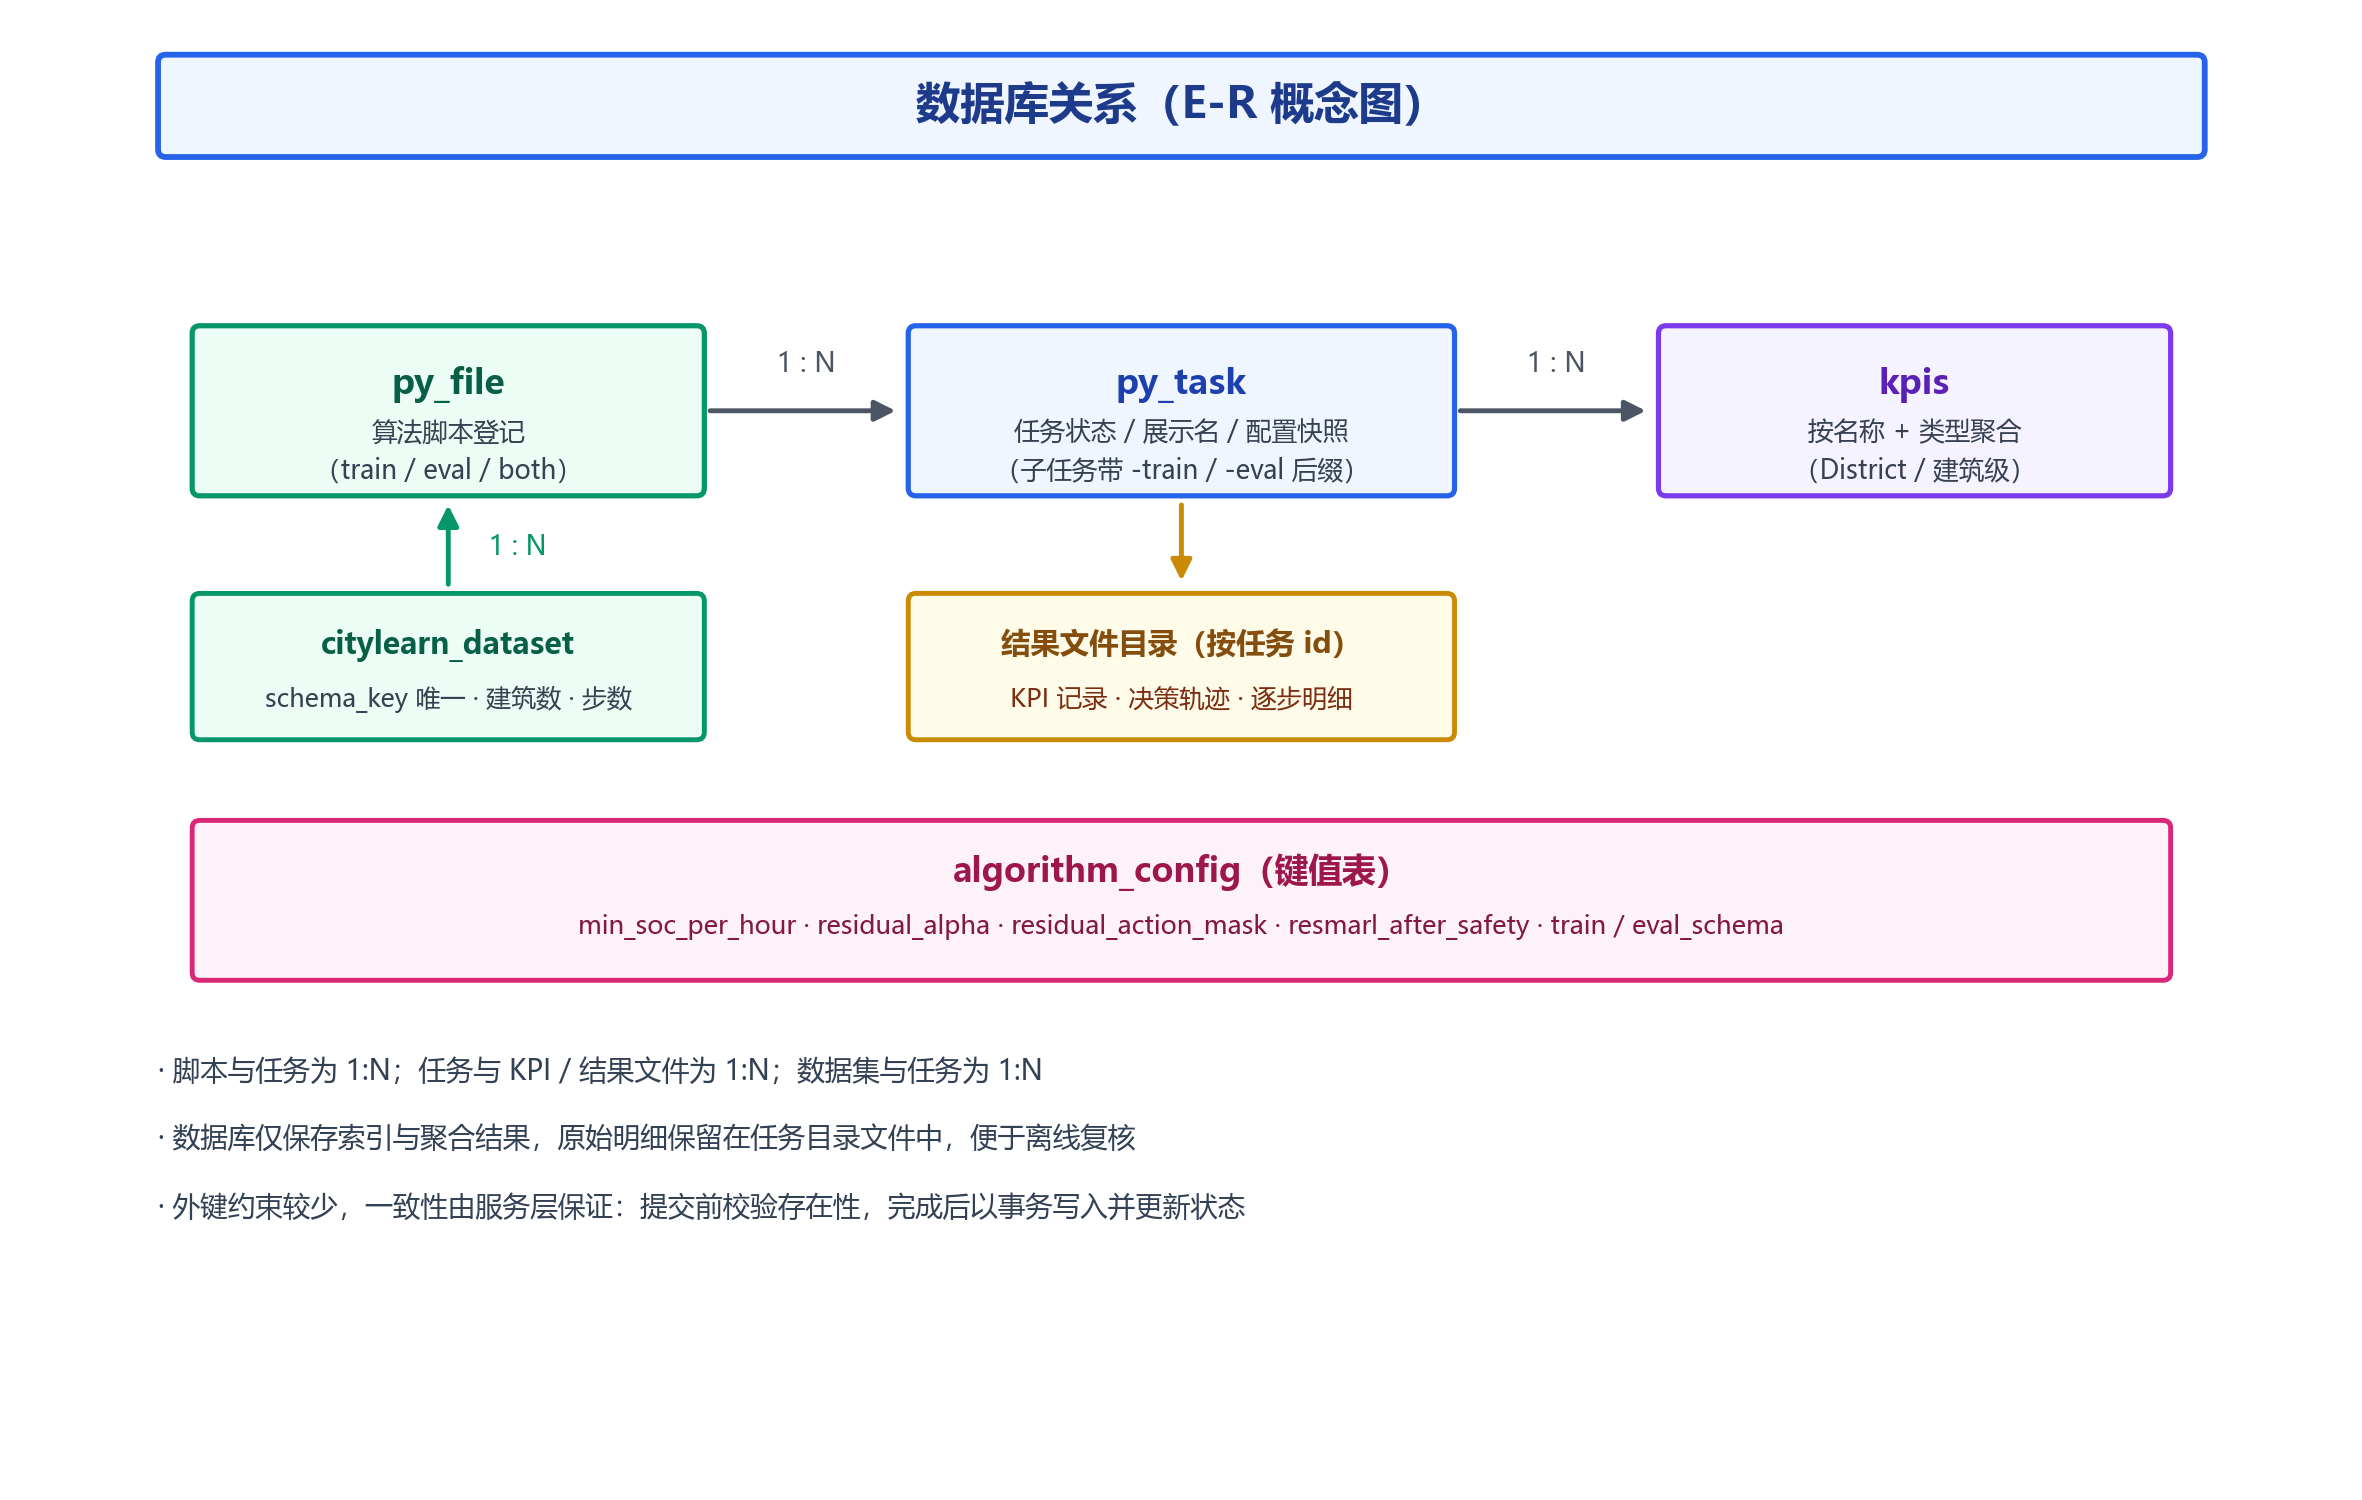
\includegraphics[width=0.85\textwidth]{./images/pictures/数据库ER图.png}
    \centering\bicaption{数据库E-R图}{E-R Diagram of the Database}
    \label{数据库E-R图}
\end{figure}

\section{本章小结}
本章将需求分析转化为架构设计：明确三类用户、四块功能、B/S四层架构，以任务标识贯通全链路。数据库概念设计先行，字段级实现详见4.3节。接口契约与日志规范是下一章的输入，Postman与日志分析的具体做法与2.4、2.5及5.1节相呼应。
